\chapter{Background}
\label{chap:background}

In this chapter, I introduce the biological concepts and methods that will be used throughout this manuscript.
I first present DNA supercoiling and its regulation in bacteria.
I outline its role in gene transcription, and the reciprocal effect of transcription on supercoiling, which jointly result in what is called the transcription-supercoiling coupling (TSC).
Then, I discuss a few cases studies in which supercoiling might have played an important evolutionary role, and that illustrate the interest of studying DNA supercoiling through the lens of evolution.
Finally, I briefly present the general method with which I tackle the questions raised in Chapter~\ref{chap:intro} throughout the manuscript.

\section{DNA Supercoiling in Bacteria}
\label{sec:background:sc}

\begin{figure}
\centering
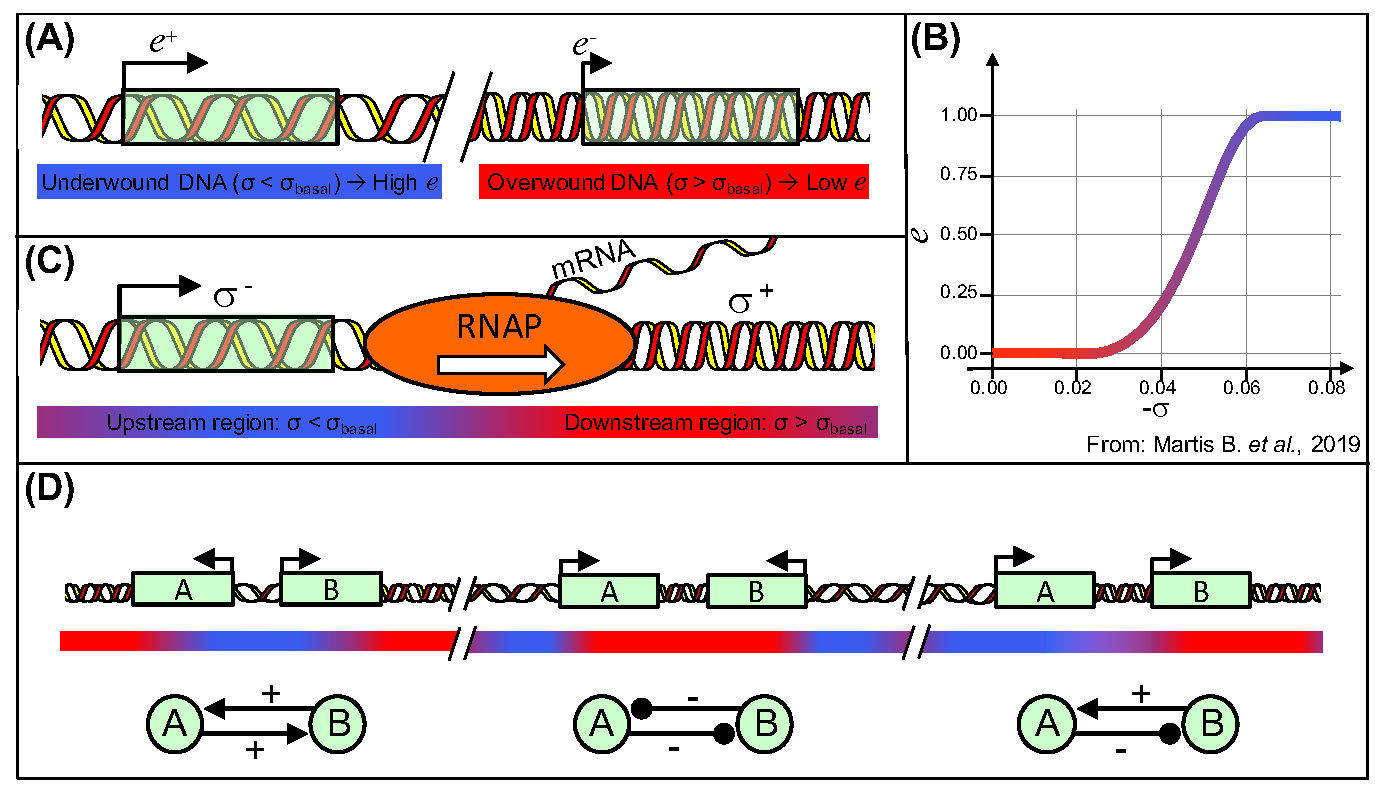
\includegraphics[width=\textwidth]{alife/img/fig-theorique.pdf}
\caption[Role of supercoiling in transcription and description of the transcription"=supercoiling coupling]{\textbf{A}. When DNA is underwound ($\sigma < \sigma_{basal}$, left), gene transcription rates are higher than when DNA is overwound ($\sigma > \sigma_{basal}$, right).
\textbf{B}. Promoter activity (equivalently, transcription level) \emph{e} increases with the level of negative supercoiling $-\sigma$.
\textbf{C}. The transcription of a gene by RNA polymerase (RNAP) generates a decrease in supercoiling upstream of the transcribed gene, and an increase downstream of the transcribed gene.
\textbf{D}. Transcription-supercoiling coupling: the sign of the interaction between neighboring genes depends on their relative orientation.
Figure reproduced from~\citep{grohens2021}.}
\label{fig:background:theory}
\end{figure}

%\paragraph{Definition of DNA supercoiling}
DNA is the material basis of genetic information.
It is a flexible polymer that comprises two strands of nucleotides that coil around each other, at a rate of 10.5 base pairs per turn in the absence of external constraints.
When subjected to torsional stress, DNA can either writhe and form 3-dimensional loops, or twist around itself more or less tightly than in its relaxed state~\citep{travers2005}; both writhing and twisting are referred to as DNA supercoiling.
The level of supercoiling is measured as the relative density $\sigma$ of supercoils in over- or under-wound DNA, as compared to relaxed DNA.
DNA is positively supercoiled ($\sigma > 0$) when it is overwound, and negatively supercoiled ($\sigma < 0$) when it is underwound.
In bacteria, DNA is normally maintained in a moderately negatively supercoiled state, with a reference value of $\sigma_{basal}=-0.06$ in \emph{Escherichia coli}~\citep{travers2005}.
In these organisms, the supercoiling level is an important regulator of gene transcription~\citep{dorman2016}.
Moreover, as transcription itself impacts DNA supercoiling~\citep{liu1987}, this results in a coupling between these two processes, of which Figure~\ref{fig:background:theory} presents an overview.
As a general rule, genes are transcribed at a higher rate when DNA is more negatively supercoiled (A), following a sigmoidal response curve (B).
Transcription generates positive and negative supercoiling downstream and upstream of transcribed genes respectively (C), resulting in a coupling between the expression levels of neighboring genes that depends on their relative orientations (D).

\subsection{Gene Regulation by DNA Supercoiling}

The level of DNA supercoiling influences gene expression, as more negatively supercoiled DNA facilitates the initiation of transcription (Figure~\ref{fig:background:theory} A).
The thermodynamical reaction of opening the DNA double strand, which is the initial step of gene transcription, is indeed favored in more negatively supercoiled DNA~\citep{elhoudaigui2019}, resulting in a sigmoidal response curve of gene expression to DNA supercoiling (Figure~\ref{fig:background:theory} B).

Due to this effect, supercoiling has experimentally been shown to act as a broad regulator of gene expression in several bacteria.
In \emph{E. coli},~\cite{peter2004} showed that 7\% of genes were sensitive to a relaxation of chromosomal DNA, of which one third were up-regulated by relaxation and two thirds down-regulated.
Similar results were obtained for \emph{S. enterica}, in which 10\% of genes were sensitive to DNA relaxation~\citep{webber2013}, and for \emph{S. pneumoniae}, in which around 13\% of genes were sensitive to relaxation~\citep{ferrandiz2010}.
When instead inducing extreme negative supercoiling in \emph{D. dadantii}, 13\% of the genes in the exponential phase and 7\% in the stationary phase were affected~\citep{pineau2022a}.

In \emph{D. dadantii}, different genomic regions moreover exhibit markedly different responses to changes in supercoiling~\citep{muskhelishvili2019}, allowing the expression of pathogenic genes only in stressful environments.
Finally, DNA supercoiling might be an especially important regulator of gene activity in bacteria with reduced genomes, such as the obligate aphid endosymbiotic bacterium \emph{Buchnera aphidicola}.
\emph{B. aphidicola} is nearly devoid of transcription factors, and supercoiling is therefore though to be one of the sole regulation mechanisms available in this bacteria~\citep{brinza2013}.

\subsection{A Dynamic DNA Supercoiling Level}

The level of DNA supercoiling in bacteria is primarily controlled by topoisomerases, enzymes that alter DNA supercoiling by cutting and rotating the DNA strands~\citep{duprey2021}.
The two main topoisomerases are gyrase, which dissipates positive supercoiling by introducing negative supercoils at an ATP-dependent rate, and topoisomerase I, which oppositely relaxes negative supercoiling~\citep{martisb.2019}.
But numerous other processes also impact the level of DNA supercoiling, either by generating new supercoils or by constraining their diffusion.

In particular, according to the twin-domain model of supercoiling~\citep{liu1987}, the transcription of a gene by RNA polymerase generates both positive and negative supercoils.
As a consequence of the drag that hampers the rotation of the RNA polymerase complex around the DNA sequence during transcription, positive supercoiling builds up upstream of the transcribed gene, and negative supercoiling downstream of the transcribed gene~\citep{visser2022}.
This phenomenon is pictured in subfigure C of Figure~\ref{fig:background:theory}.
Moreover, while the intrinsic flexibility of the DNA polymer would in principle allow supercoils to propagate freely along the chromosome, many nucleoid-associated proteins such as FIS, H-NS or HU bind to bacterial DNA~\citep{krogh2018}, in addition to RNA polymerases.
These DNA-bound proteins create barriers that block the diffusion of supercoils, resulting in what have been termed topological domains of supercoiling~\citep{postow2004}.

The level of DNA supercoiling can furthermore be affected by numerous environmental stresses in bacteria.
Salt shock transiently increases negative DNA supercoiling in \emph{E. coli}~\citep{hsieh1991}; the acidic intracellular environment relaxes DNA in the facultative pathogen \emph{Salmonella enterica} var. Typhimurium~\citep{marshall2000}; and higher temperatures relax DNA in the plant pathogen \emph{Dickeya dadantii}~\citep{herault2014}.
These constraints overall paint the picture of a very dynamic DNA ``supercoiling landscape'' in bacteria~\citep{visser2022}, with a supercoiling level that varies in both time and space during the bacterial lifecycle and along the chromosome.

\subsection{Supercoiling and Evolution}

Gene regulation by DNA supercoiling can itself be subject to evolution by natural selection, as a mechanism by which to adapt gene expression levels to new environments.
In the \emph{Long-Term Evolution Experiment} (\emph{LTEE})~\citep{lenski1991}, 12 populations of \emph{E. coli} have been maintained for over 80,000 generations, evolving and adapting to a glucose-limited environment.
In 11 of the 12 populations in the experiment, an increase in fitness was linked to mutations in genes which participate directly or indirectly in the regulation of the supercoiling level, such as \emph{topA}, \emph{fis}, or \emph{dusB}~\citep{crozat2010}.
When inserted into the ancestral strain, the mutant \emph{topA} and \emph{fis} alleles increased the level of negative supercoiling as well as the bacterial growth rate, demonstrating
that supercoiling mutations can play a role in the adaptation to new environments through their broad regulatory effect~\citep{crozat2005}.
From an epistasis perspective, the repeated fixation of supercoiling mutations in the \emph{LTEE} suggests that these mutations could confer an evolutionary advantage to the lineages in which they appear by favoring the apparition of compensatory mutations in supercoiling-regulated genes; but this possible epistatic role should nonetheless be disentangled from their direct fitness effect in order to conclude with more certainty.

The regulation of gene expression by DNA supercoiling could moreover be a force that participates in shaping the evolution of the organization itself of bacterial genomes.
Indeed, supercoiling"=sensitive genes tend to group in up or down-regulated clusters in \emph{E. coli}~\citep{peter2004}, \emph{S. enterica}~\citep{webber2013} and \emph{S. pneumoniae}~\citep{ferrandiz2010}.
This suggests the possibility of a phenotypic role in the co-localization of genes in these clusters, through a common regulation of their transcription~\citep{sobetzko2016}.
Synteny segments, or clusters of neighboring genes that show correlated expression patterns, are indeed evolutionarily conserved across \emph{E. coli} and the distantly related \emph{Bacillus subtilis}, strengthening the hypothesis that these domains could play an important role in the regulation of bacterial gene expression through supercoiling-mediated interactions~\citep{junier2016}.


\section{The Transcription-Supercoiling Coupling}

As shown in Figure~\ref{fig:background:theory}C, the transcription of a given gene by an RNA polymerase generates an accumulation of positive supercoiling downstream of that gene, and of negative supercoiling upstream of that gene, because of the hindered movement of the polymerase~\citep{liu1987,visser2022}.
If a second gene is located closely enough to this first gene on the genome, the change in supercoiling at the promoter of the second gene will impact the transcription rate of that gene, as negative supercoiling usually facilitates gene transcription~\citep{forquet2021}.
In turn, the transcription of the second gene will also generate a local change in supercoiling that affects the first gene, resulting in an interaction between the transcription levels of these two genes, which has been called the transcription-supercoiling coupling~\citep{meyer2014}.
Depending on the relative orientation of these genes, the coupling can take several forms.
Divergent genes increase their respective transcription level in a positive feedback loop; convergent genes inhibit the transcription of one another; and in tandem genes, the transcription of the downstream gene increases the transcription of the upstream gene, while the transcription of the upstream gene decreases the transcription of the downstream gene.

This supercoiling-mediated interaction between neighboring genes has been documented in several bacterial genetic systems.
In the \emph{E. coli}-related pathogen \emph{Shigella flexneri}, the \emph{virB} promoter is normally only active at high temperature, but can be activated at low temperature by the insertion of a phage promoter in divergent orientation~\citep{tobe1995}.
Similarly, the expression of the \emph{leu-500} promoter in \emph{S. enterica} can be increased or decreased by the insertion of upstream transcriptionally active promoters, depending on their orientation relative to \emph{leu-500}~\citep{elhanafi2000}.
The magnitude of the effect of the transcription-supercoiling coupling has also been explored in a synthetic construct, in which the inducible \emph{ilvY} and \emph{ilvC} \emph{E. coli} promoters have been inserted on a plasmid in divergent orientations.
In this system, a decrease in the activity of \emph{ilvY} is associated with a decrease in \emph{ilvC} activity, and an increase in \emph{ilvY} activity with an increase in \emph{ilvC} activity as well~\citep{rhee1999}.

There are, however, hints that the biological relevance of the transcription-supercoiling coupling might not be confined to these few specific instances.
Indeed, in \emph{E. coli}, the typical size of topological domains -- inside which the positive and negative supercoils generated by gene transcription can propagate -- is usually estimated to measure around 10 kb~\citep{postow2004}, while transcription-generated supercoiling could propagate up to 25 kb in each direction around a transcribed gene~\citep{visser2022}.
As genes measure on average 1~kb and intergenic distances 120 bp in \emph{E. coli}~\citep{blattner1997}, any single topological domain on the \emph{E. coli} chromosome therefore encompasses multiple genes that can potentially interact via the transcription-supercoiling coupling.
A statistical analysis of the relative position of neighboring genes on the \emph{E. coli} chromosome indeed shows that genes that are up-regulated by negative supercoiling have more neighbors in divergent orientations, while genes that are down-regulated by negative supercoiling have more neighbors in converging orientations~\citep{sobetzko2016}, further suggesting that the transcription-supercoiling coupling plays a role in regulating the activity of genes located in the same topological domain.


\section{Existing Models of the Transcription-Supercoiling Coupling}

Several mathematical and computational models have been proposed to describe the effect of the transcription-supercoiling coupling on the expression level of neighboring genes.
In~\cite{meyer2014}, a quantitative model of the supercoiling level at a locus of interest is proposed, in order to study the transcription-supercoiling coupling between a pair of adjacent genes.
In that model, DNA transcription is regulated by the opening free energy of DNA around gene promoters, which directly depends on the supercoiling level.
The reciprocal influence of neighboring genes is then obtained by computing the difference in transcription levels due to supercoiling and the subsequent variation in supercoiling, and iterating this system until a fixed point is reached.
A more detailed stochastic model is presented in~\cite{elhoudaigui2019}.
This model aims at making quantitative predictions of gene expression levels, and introduces explicit RNA polymerases and topoisomerases that delineate dynamic supercoiling domains inside which supercoils immediately propagate.
In that model, the transcription level of a genomic region of interest is simulated using discrete time steps, during which RNA polymerases attach to the DNA template, progress along the transcribed region while generating positive supercoiling in the downstream domain and negative supercoiling in the upstream domain, and finally detach from DNA, merging the two domains separated by the polymerase.

Another family of biophysical models aim at describing the movement of RNA polymerases along the genome during gene transcription, and therefore model the level of DNA supercoiling, as supercoils impact the speed at which polymerases can progress forward.
In~\cite{brackley2016}, a stochastic model of the transcription of co-oriented genes is proposed, in order to study transcriptional bursts.
This model is qualitatively different from the models presented above, as it explicitly models the level of supercoiling as a function of time and of the position along DNA, whereas the former models consider it as constant in the intervals delimited by polymerases or NAPs.
A similar model is introduced in~\cite{sevier2017}, in order to study the possible stalling of DNA polymerases due to excessive transcription-generated supercoiling in a single gene.
This second model has then been extended to accommodate the supercoiling-mediated interaction of neighboring genes in~\cite{sevier2018}, making qualitatively similar predictions of gene transcription rates as the first set of models presented above.
This model has finally been used to propose a toggle switch~\citep{gardner2000} in which gene regulation by transcription factors is replaced by regulation by transcription-generated supercoiling~\citep{sevier2021}.

The common limit to all the models described above is that these models focus on mechanistic descriptions of the supercoiling-mediated local interaction between neighboring genes, but do not try to generalize to the whole-genome scale nor to an evolutionary time frame.
Exploring the role of the transcription-supercoiling coupling at the scale of complete bacterial genomes, and the reaction of supercoiling-mediated interactions to the changes in relative gene positions that can be caused by genomic rearrangement, however seems necessary in order to decipher the evolutionary role of supercoiling mutations.


\section{An Evolutionary Systems Biology Approach}

The models of the transcription-supercoiling coupling presented above demonstrate that the system that emerges from the coupled transcription of neighboring genes on a genome is complex, in the sense that it presents behaviors that cannot be explained by modeling each gene in isolation.
Moreover, studying the epistatic interactions between mutations in genes that regulate supercoiling and in genes that are regulated by supercoiling requires the addition of another layer of complexity, as the effect of supercoiling mutations or genomic rearrangements on gene transcription levels cannot be directly predicted from the mutations themselves.
In order to tackle this problem, I followed the methodological approach of evolutionary systems biology, which adapts the tools of systems biology to study not only complex systems themselves but also their evolution -- in the Darwinian sense -- over time, with the help of computer simulations~\citep{beslon2021}.

\begin{figure}
\centering
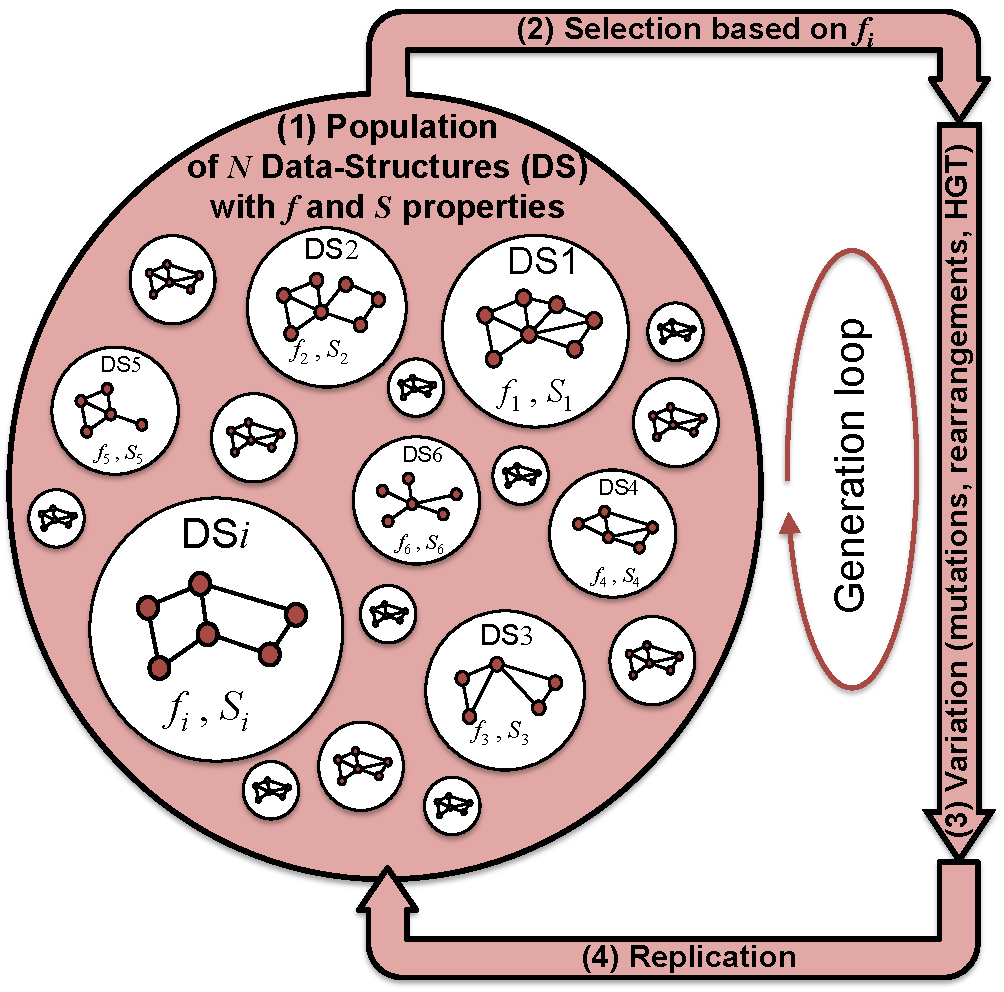
\includegraphics[width=0.75\textwidth]{background/img/evol_sys_bio.pdf}
\caption[Template of an evolutionary systems biology simulation]{Template of an evolutionary systems biology simulation.
In a population of complex systems, each individual $i$ is represented by an inner data structure $DS_i$, from which systemic properties of interest $S_i$ emerge, and that is used to compute a fitness level $f_i$.
The population can then evolve by following an evaluation-selection-variation-replication loop.
Figure reproduced with permission from~\citep{beslon2021}.}
\label{fig:background:evol-sys-bio}
\end{figure}

The core of this approach is represented in Figure~\ref{fig:background:evol-sys-bio}, which describes the evolution of a population of complex systems, or ``digital organisms''~\citep{adami2006}.
Each complex system in the population is represented by the means of a data structure $DS_i$, which represents an instantiation of underlying system with a particular set of parameter values.
Using this data structure, we can evaluate the systemic properties of interest $S_i$ of this individual, and its fitness value $f_i$.
A new population of complex systems can then be created by selecting reproducers based on fitness, and making their underlying data structure undergo stochastic mutations that can affect both their systemic properties and their fitness.
This cycle can then be repeated for a given number of generations, resulting in an experimental framework called ``\emph{in silico} experimental evolution'', as it adapts the traditional \emph{in vivo} experimental evolution methodology to the computational study of the evolution of arbitrary complex systems.

Both \emph{Aevol} (introduced in Chapter~\ref{chap:aevol}) and \emph{EvoTSC} (introduced in Chapter~\ref{chap:alife}), the \emph{in silico} artificial evolution platforms that I developed and used during my PhD, follow this methodology.
In both platforms, each complex system represents a given individual which is described by its genome; the models diverge in the data structure with which they represent genomes, as \emph{Aevol} is a nucleotide-level model whereas \emph{EvoTSC} is a ``string-of-pearls'' model, in which genomes are represented by a series of genes separated by non-coding sections (see~\cite{hindre2012} for an overview of these formalisms).
The fitness of individuals is obtained in both platforms by evaluating their gene transcription levels, and comparing these transcription levels to an implicit (in \emph{Aevol}) or explicit (in \emph{EvoTSC}) target.
Finally, the systemic properties of individuals differ in each model, according to their choice of underlying data structure: \emph{Aevol} can be used to study properties such as genome size or the proportion of coding bases, whereas \emph{EvoTSC} can be used to study the arrangement of genes on the genome.


\section{Conclusion}

The level of DNA supercoiling is an interesting property of bacterial genomes, standing at the crossroads of many processes: it is finely regulated by the joint action of topoisomerases and nucleoid-associated proteins, but remains sensitive to the external influence of environmental stress, and to the internal influence of gene transcription.
The repeated mutations targeting the regulation of the supercoiling level in the \emph{LTEE} demonstrate the role that supercoiling can play -- through its central position in genome biology -- in the adaptation of bacterial populations to new environments, and make it an ideal example to study the role of epistatic interactions in guiding evolutionary trajectories.
Moreover, as gene transcription itself depends on DNA supercoiling, the resulting interplay between transcription and supercoiling generates a complex web of interactions between neighboring genes in the dense bacterial genomes: the transcription-supercoiling coupling.
While the effect of this coupling has already well been studied at the scale of a few neighboring genes, expanding this analysis to the whole-genome scale seems necessary in order to have a qualitative understanding of the phenotypic consequences of supercoiling mutations, and hence of their possible epistatic interactions.

Finally, an \emph{in silico} experimental evolution approach seems to be the most promising way to tackle the study of the evolutionary role of these mutations, as this methodology enables the combination of a complex model of the transcription-supercoiling coupling -- an integral part of gene regulation by DNA supercoiling -- with an evolutionary model that allows for the emergence of complex epistatic interactions that can influence evolutionary trajectories.
